\subsection{Определение коррекций задержек между каналами}\label{section:Corrections}

Типичная гистограмма разности временных отметок передних фронтов, соответствующих фотонам из одной вспышки лазера, зарегистрированных в заданной паре каналов, показана на \figref{fig:TypicalLeadingEdgeDiff}. Такие гистограммы позволяют определить положение пика и, соответственно, ввести коррекцию задержки. Отметим, что наблюдается дрейф порядка 0,5~нс значений задержек, полученных таким образом, что даёт заметный вклад во временное разрешение системы считывания (см.~секцию~\ref{section:TimeRes}).

Наблюдается также аддитивность задержек, т.е. задержка в i-м канале относительно опорного может быть получена с точностью не хуже 400~пс как сумма задержки в j-м канале относительно опорного и задержки в i-м канала относительно j-го. Для некоторых пар каналов вид гистограммы отличается от показанной на \figref{fig:TypicalLeadingEdgeDiff}. См., например, \figref{fig:LeadingEdgeDiffMultiplePeaks}. Подобное распределение можно получить, если один из двух каналов является дефектным в том смысле, что к фронту логического сигнала подмешивается возбужденный или наведённый колебательный сигнал. Такая гипотеза подтверждается тем фактом, что форма гистограммы зависит от порога дискриминатора на плате PADIWA. При построении аналогичной гистограммы для пары дефектных каналов наблюдается до 5~пиков. Дальнейшее исследование проводилось с исключением дефектных каналов. Доля дефектных каналов составляет около 10\% от полного числа каналов. При разработке следующей версии передней электроники для CBM RICH особое внимание будет уделено электромагнитной чистоте каналов, а гистограммы, подобные обсуждаемым в данном разделе, будут использоваться в качестве диагностического инструмента.

\begin{figure}[H]
\centering
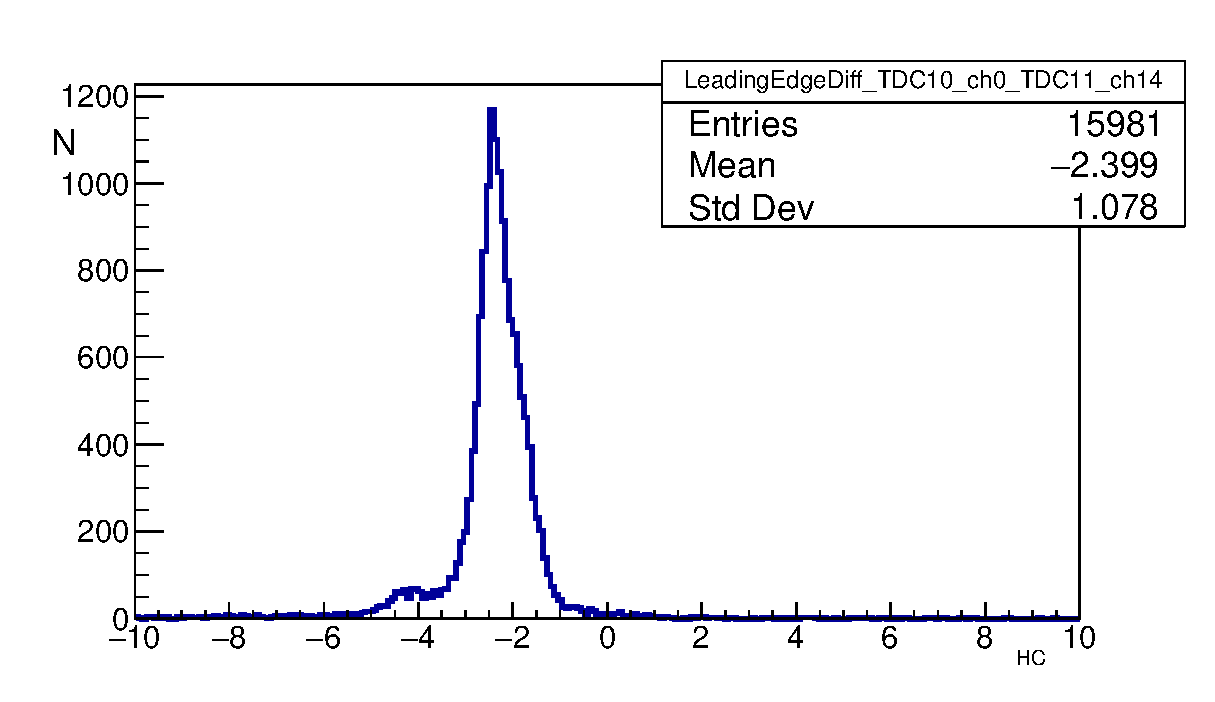
\includegraphics[width=1.0\textwidth]{pictures/22_LeadingEdgeDiff_TDC10_ch0_TDC11_ch14_feb2017.eps}
\caption{Распределение разности временных отметок передних фронтов, соответствующих фотонам из одной вспышки лазера, зарегистрированных в заданной паре каналов.}
\label{fig:TypicalLeadingEdgeDiff}
\end{figure}

\begin{figure}[H]
\begin{minipage}[b]{0.495\textwidth}
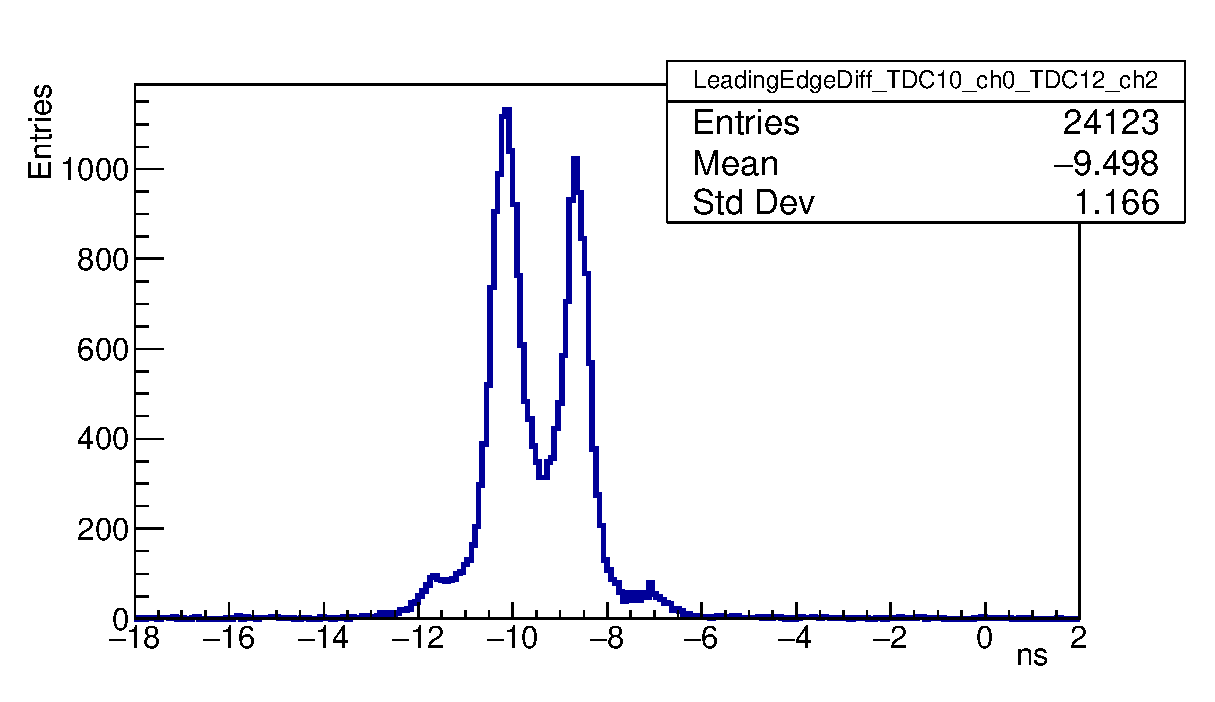
\includegraphics[width=1.0\textwidth]{pictures/23_LeadingEdgeDiff_TDC10_ch0_TDC12_ch2_feb2017.eps}
\end{minipage}
\hspace{0.01\textwidth}
\begin{minipage}[b]{0.495\textwidth}
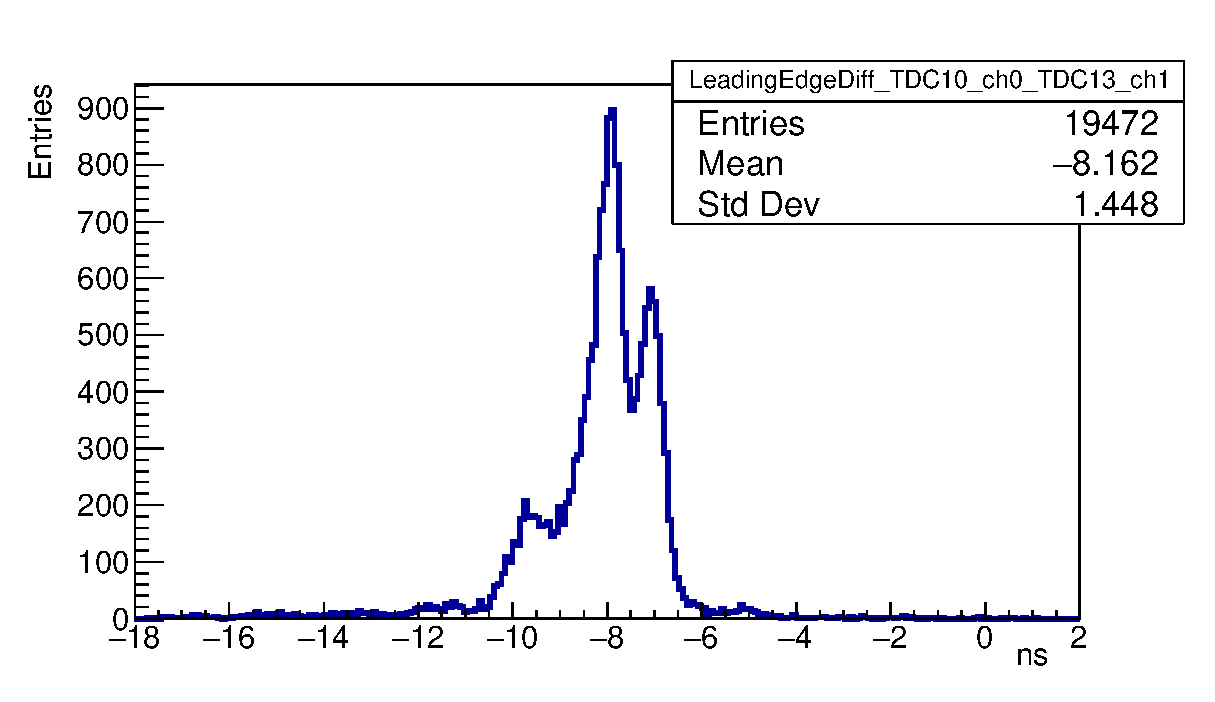
\includegraphics[width=1.0\textwidth]{pictures/23_LeadingEdgeDiff_TDC10_ch0_TDC13_ch1_feb2017.eps}
\end{minipage}
\caption{Распределение разности временных отметок передних фронтов, соответствующих фотонам из одной вспышки лазера, зарегистрированных в заданной паре каналов, при условии, что один из каналов --- дефектный.}
\label{fig:LeadingEdgeDiffMultiplePeaks}
\end{figure}

%\begin{figure}[H]
%\includegraphics[width=1.0\textwidth]{pictures/}
%\caption{}
%\label{fig:}
%\end{figure}
